\chapter{The nEDM active magnetic shielding}

\label{ch:nedm_sfc}
In this chapter the principle of an active magnetic shielding is explained, followed by a description of the system of the PSI nEDM experiment. The matrix-based feedback algorithm and the properties of the matrix are discussed. Finally, the challenges for the design of a next-generation system for the n2EDM experiment at PSI are stated.




\section{The principle of active magnetic shielding}
Passive methods of shielding the magnetic field, like mu-metal shields, rely on magnetic properties of materials. In contrast, in active methods the disturbances are first detected, processed and then counteracted. It is not unlike the recently popular active-noise-cancellation headphones. Standard ones provide only passive damping of the ambient noise by covering the ears. Active headphones additionally feature microphones that resolve the profile of incoming sound, which is then inverted and emitted from the speakers. The two waveforms, when overlaid, cancel.

\begin{figure}
  \centering
  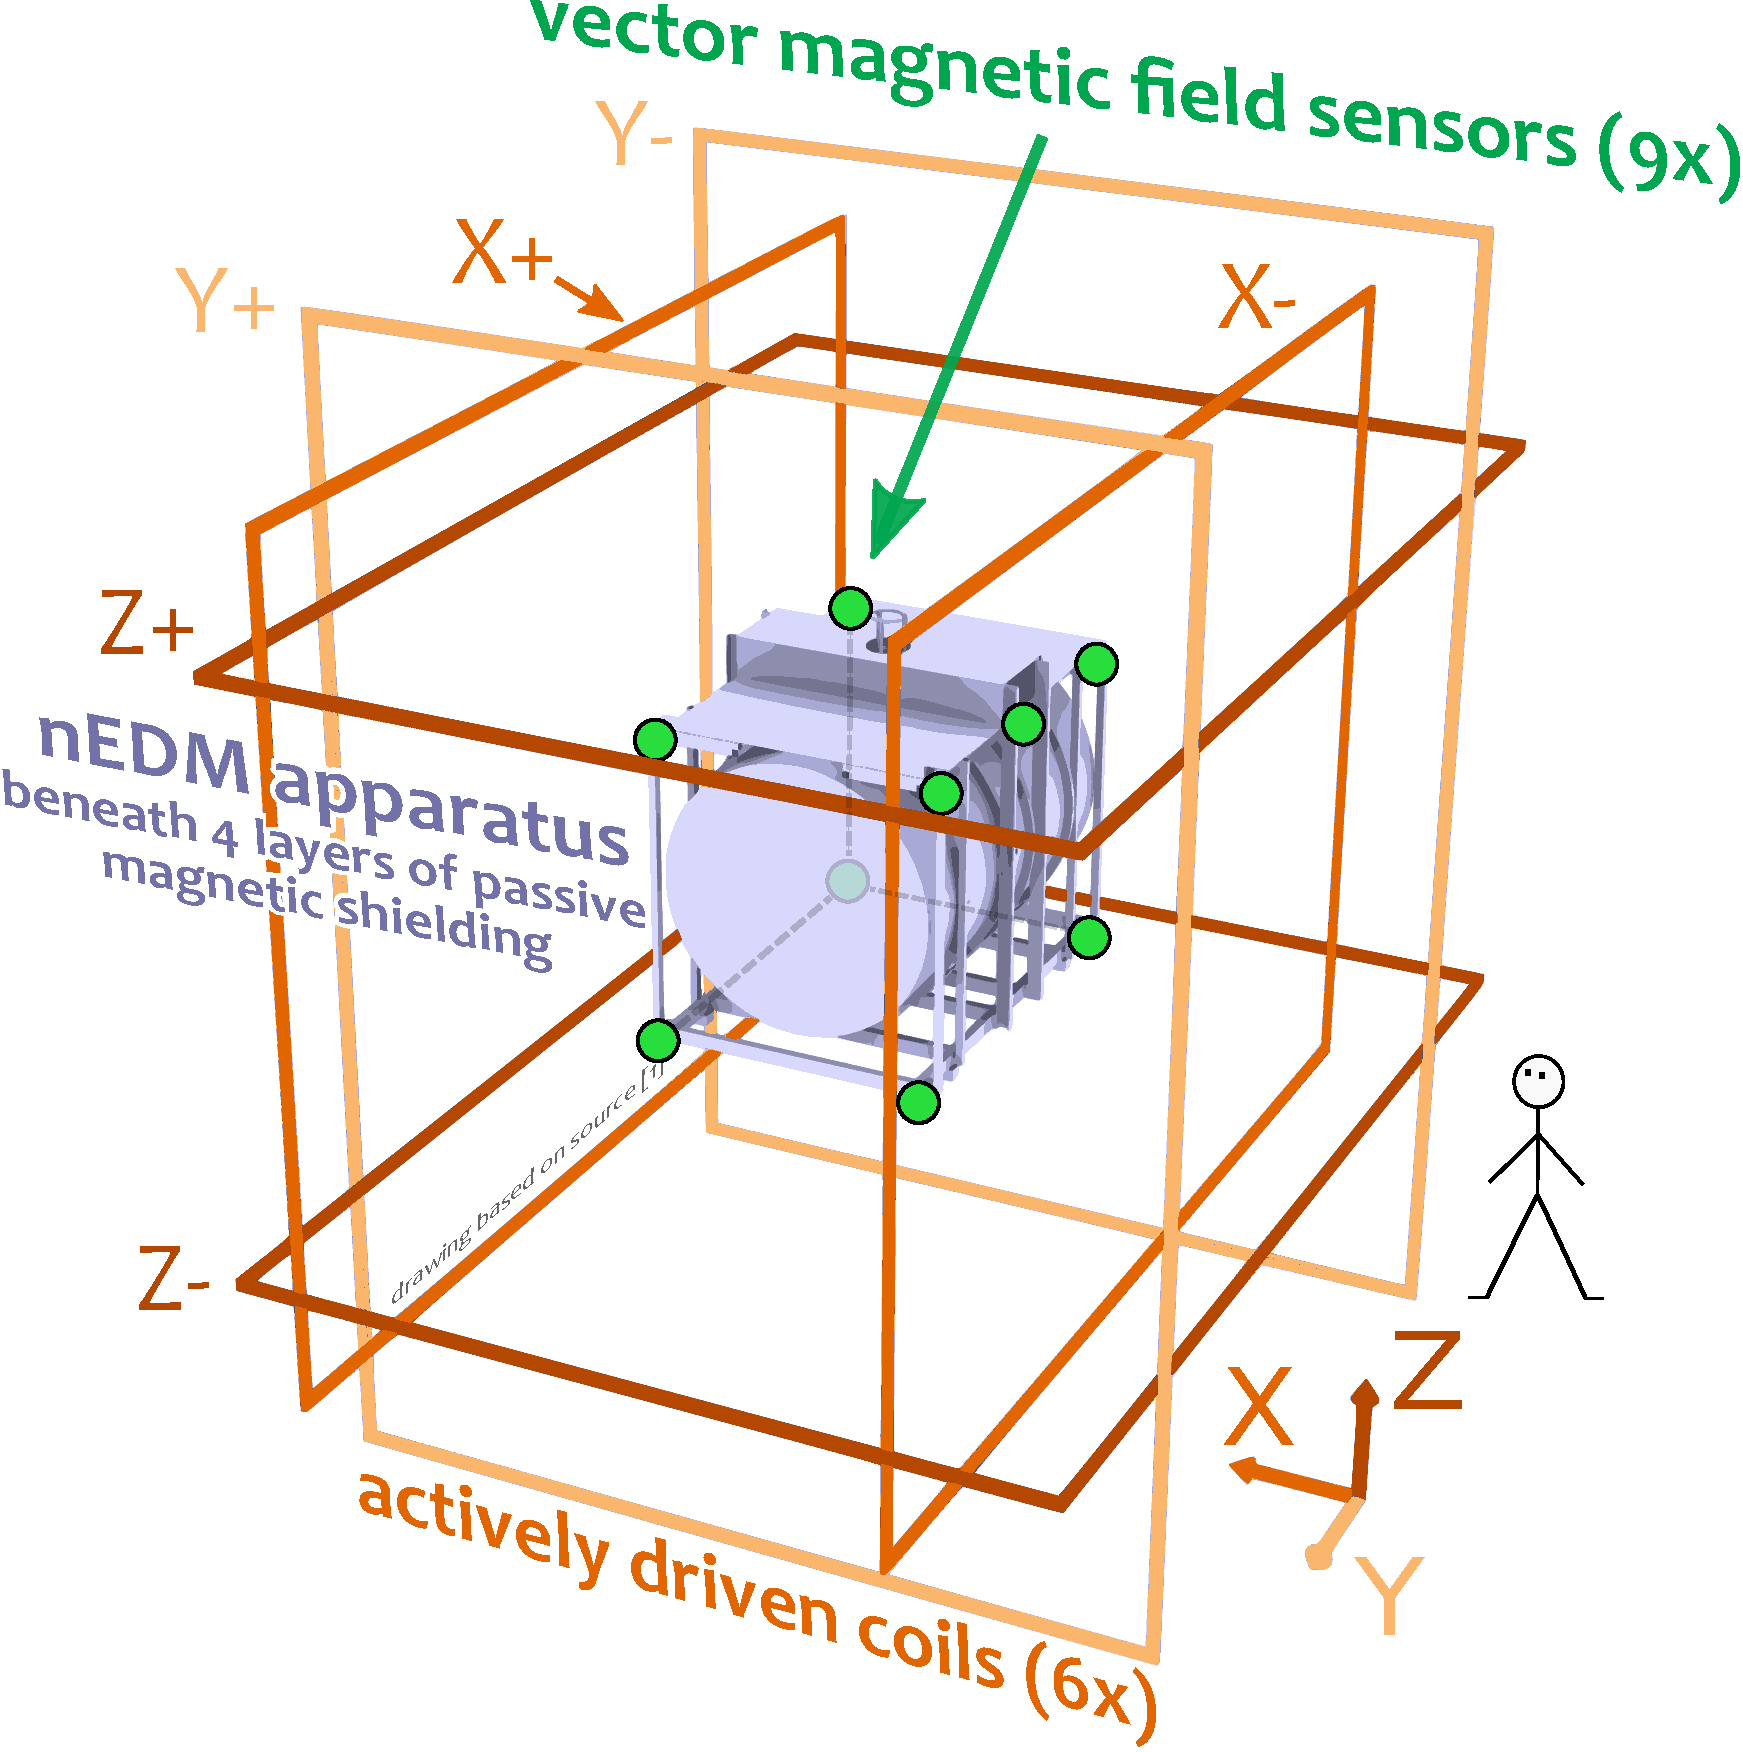
\includegraphics[width=0.8\linewidth]{gfx/nEDM_SFC/SFC_scheme.pdf}
  \caption{The nEDM at PSI active magnetic shield (SFC). The experiment, in violet, was in the middle, with nine 3-axis magnetic field sensors, depicted as green circles, attached to it. Everything was encircled by six coils (orange). Adapted from~\cite{Franke2013}.}\label{fig:sfc-scheme}
\end{figure}

Active magnetic shields follow the same principle. A volume, often called the fiducial volume, is encircled by coils. Within the volume magnetic field sensors are distributed. It is schematically presented in Fig.\,\ref{fig:sfc-scheme}, taking the PSI nEDM experiment's system as an example. The fiducial volume is filled with the violet structure in the middle (the passive shield). The green dots depict the magnetic field sensors. Around there are three orthogonal Helmholtz-like pairs of coils, depicted in shades of orange. The sensors detect the variations of the magnetic field, an appropriate counteraction is calculated and currents are applied to the coils.

Active shields do not substitute passive ones.
The shielding factor
\marginpar{Shielding factor, measured in \si[detect-all=true]{\decibel} is a tenth of the logarithm of the ratio of the power of the magnetic field as if it were not compensated to the compensated one.}
of passive shields degrades for frequencies slower than \SIrange[range-phrase = --]{1}{10}{\hertz}~\cite{Brake1991,PTBroom}.
% The loss in the shielding factor can be as much as \SI{70}{\decibel} (three orders of magnitude in amplitude of the field).
At the same time active systems perform best at DC and reach up to the kilohertz regime.
The combination of the two shielding methods provides a stable magnetic field over the whole range of frequencies~\cite{Brake1991,Kelha1982,PTBroom,Voigt2013}.

Since the 1980s numerous active shields have been built~\cite{Kelha1982,Brake1991,Spemann2003,Brys2005,Kobayashi2012,Voigt2013,Afach2014}. The applications span from ion beams, through bio-magnetism, all the way to nEDM measurements, in particular the one conducted at PSI\@.

% \note{Don't discuss it here: In the overlapping range of frequencies, where the two kinds of magnetic shielding could compete, the two advantages of the active shielding would certainly be the cost and accessibility of the enclosed volume.}



\marginpar{There was an inside joke that SFC really stands for SULTAN Field Compensation, SULTAN having been the magnet with by far the strongest influence on the magnetic field.}
\section{The nEDM at PSI SFC system}
The construction of an active shield for the nEDM measurement at PSI, called the SFC (Surrounding Field Compensation) system,
was a part of Beatrice Franke's PhD thesis~\cite{Franke2013}, later also published~\cite{Afach2014}.

% In this section the SFC system is presented, fo
% In the beginning of this chapter the most important information about the SFC system is presented, followed by a few new insights. This serves as an introduction to the original developments, to which the remaining three chapters of part II are dedicated.

The distinct feature of the PSI's SFC system was the use of a feedback matrix.
\marginpar{A matrix-based feedback was first proposed by~\cite{RetaHernandez1998}. As their proposed system did not include $\mu$-metal, they could calculate the matrix analytically.}
Consider a single coil of any shape in air. For every point in space, and for every spatial component, the magnetic field is directly proportional to the current in the coil. The SFC system had six coils and measured the field in nine points, three spatial components in each. In total there were $6 \times 27 = 162$ proportionality constants, which were gathered in the feedback matrix $M$. The matrix $M$ is a property of the active compensation system, more precisely of the geometry of the coils and sensors. It could have been calculated analytically, if not for the mu-metal shield. Ferromagnetic materials distort the magnetic field around them.
Different to similar systems~\cite{Kelha1982,Brake1991,Spemann2003,Brys2005,Kobayashi2012,Voigt2013}, which used independent feedback for each coil, the SFC system at PSI used the matrix $M$ that mixes all sensors and all coils. 
% The use of the matrix $M$ was what distinguished the PSI's SFC system from other systems~\cite{Kelha1982,Brake1991,Spemann2003,Brys2005,Kobayashi2012,Voigt2013}, which used either one component of a sensor, or a weighted combination of several components, to control one coil.

% Moreover, they make the system non-linear, which we are going to, for now, neglect.

% \note{Maybe some nice formula here for the matrix elements?}

\begin{figure}
  \centering
  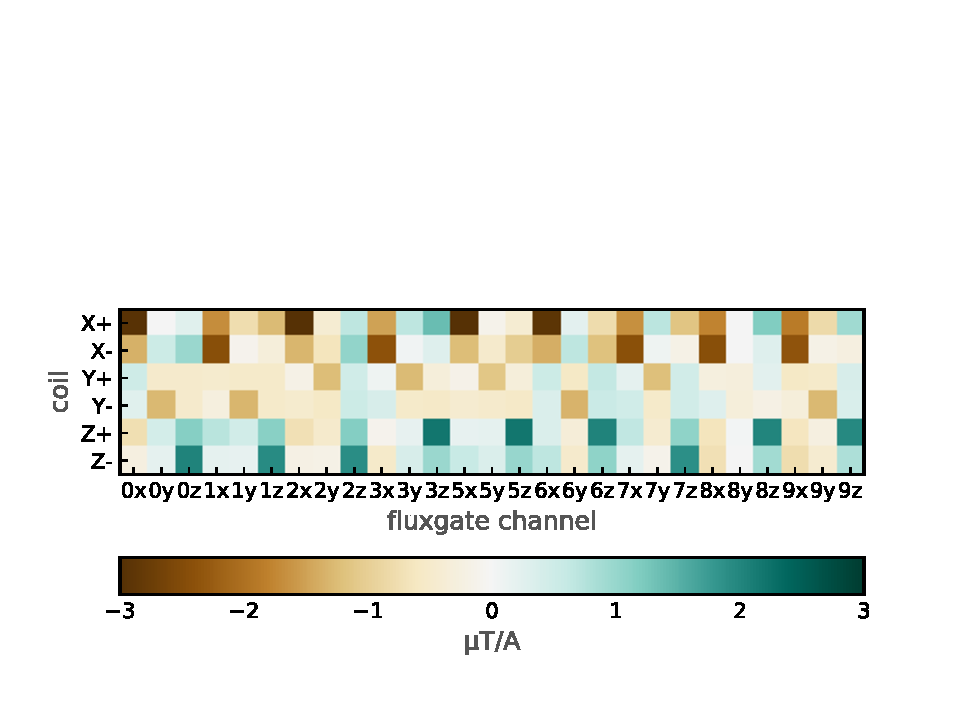
\includegraphics[width=.8\linewidth]{gfx/nEDM_SFC/nEDM_SFC_matrix.pdf}
  \caption{The SFC matrix measured by Franke on 2012--11--07~\cite{Franke2013}. For each coil (rows) and each channel of the magnetic field measurement (columns) the proportionality constant between the current in the coil and the field measured by the sensor is depicted. The coils and the sensors are labelled as in Fig.\,\ref{fig:sfc-scheme}.}\label{fig:nEDM_SFC_matrix}
\end{figure}

To measure the matrix the following procedure was used: A current in one coil was scanned in steps over the whole available range, while the field change was measured with the sensors. Then for each sensor, and each spatial component, a linear regression was performed. The slope corresponded to the proportionality constant, an element of the matrix $M$. The procedure was repeated for all coils. The matrix measured by Franke is depicted in Fig.\,\ref{fig:nEDM_SFC_matrix}.




\section{The feedback algorithm}
The PSI's SFC system followed the established norm~\cite{Kelha1982,Brake1991,Spemann2003,Brys2005} and used a PID loop to control the currents. (PI in this particular case, the derivative term was not used.) The $j$th current in the $n$th iteration was~\cite{Franke2013}:
\begin{equation}
  \label{eq:old_SFC_feedback}
  I^n_j = I^0_j +
    \underbrace{ \alpha^\mathcal{P}_j \, \Delta I^n_j }_\text{proportional term} +
    \underbrace{ \alpha^\mathcal{I}_j \, \sum_m \Delta I^m_j }_\text{integral term} \ .
\end{equation}

% $\Delta I^n_j$ is the error value in the current space. It was obtained by using the error value in the field space (the difference of the measured and target fields) and transforming it into the current space with the pseudoinverse of the matrix~\cite{Franke2013}:
\marginpar{The SFC system, when started, was static. Then the currents could be changed manually to achieve a desired field (or chosen from a predefined set). Then the system was switched to the dynamic mode~\cite{Franke2013}.}
$\Delta I^n_j$ is the error value. It was obtained from the deviation of the measured and target field, $\Delta B^n_{k'}$ for the $k'$th sensor, by multiplying it by the pseudoinverse of the matrix $M$, denoted $M^\dagger$~\cite{Franke2013}:
\begin{equation}
  \Delta I^n_j = \sum_{k'} M^\dagger_{jk'} \, \Delta B^n_{k'} \ .
\end{equation}

Besides the proportional and integral terms, the feedback formula also included the $I^0_j$ term. It may seem puzzling to give such a big of a role to particular currents that had happened to be there at the zeroth iteration. The reason behind this choice was a particular property of the SFC system: the target field was always the one measured at the moment of switching the system from the dynamic mode (feedback running) to the static one (static current output).
At that moment the error value was zero, and so was the integral term, so, according to the Eq.\,\ref{eq:old_SFC_feedback}, the output currents would immediately have switched to zero. In result the system would violently destabilise. The additional term $I^0_j$ prevented that from happening.

Here we conclude the brief description of the system and proceed to present original insights of the author.




\section{Interpretation of the feedback matrix}
There is a fundamental meaning behind the matrix $M$. The currents in the six coils can be gathered into a vector $\mathbb{I}$ in a space we call the \emph{current space}. Similarly, the 27 readouts of the magnetic field can be gathered into a vector $\mathbb{B}$ in the \emph{field space}. Then, the matrix $M$ provides the transition from the current into the field space. In particular, we have:
\begin{equation}
  \mathbb{B} = M \mathbb{I} + \mathbb{B}_\text{offset} \ .
\end{equation}
\marginpar{Finding the pseudoinverse of a matrix $A$ is equivalent to finding least-squares solution of a system of linear equations described by the matrix $A$ (although computationally more complex).}
Which is read: The measured values are a linear combination of the currents in the coils plus the ambient field.
The other direction, from the field to the current space, cannot be done exactly. Nevertheless, the optimal, in the least-squares sense, transition can be done with the use of the Moore-Penrose inverse (pseudoinverse) of the matrix $M$, denoted $M^\dagger$~\cite{penrose_1955}.
In other words, the matrix $M$ tells us what field, as measured by the sensors, a given set of currents will produce. The matrix $M^\dagger$ tells us, what currents to apply to best approximate a given field.




\section{The spectrum of the feedback matrix}
\label{sec:nedm_sfc_matrix}
The feedback matrix used during the data taking of the nEDM PSI experiment at PSI (2014--17) was the one measured by Franke (Fig.\,\ref{fig:nEDM_SFC_matrix}). The inverse of the matrix was regularised~\cite{Franke2013}. Let us now elaborate on regularisation.
% While it has been thoroughly discussed how to do the regularisation, the question of why was it needed at all was neither posed nor answered.

The feedback matrix represents coefficients in a system of linear equations that need to be solved in order to make the optimal transition from the field to the current space.
As the system of equations is over-determined, the best solution is found by the least-squares.
This is equivalent to calculating the pseudoinverse matrix. A solution can be found reliably if the system is well-defined, i.e.\ the least-squares well is steep in every direction in the parameter space.
If the well stretches, like a valley, in some directions, the solution is not globally well-defined.
Still, it may be defined up to a parameter, the one pointing along the direction of the valley.
We then speak of an ill-defined set of equations, or an ill-defined matrix.
Regularisation helps an ill-defined problem to become better defined, at the cost of the solution having larger sum of the residuals squared.

The \emph{Singular Value Decomposition} (SVD) of a real matrix $M$ is
\begin{equation}
  M = U S V^T \ , 
\end{equation}
where $U$ and $V$ are unitary, and $S$ is diagonal~\cite{Golub1965}. The singular values lie on the diagonal of $S$, which is called the \emph{spectrum}. 
% The spectrum of the feedback matrix is of uttermost importance.
Pseudo-inverting a matrix with small singular values is an ill-posed problem. Similarly, as inverting small numbers.

The \emph{condition number} of a matrix is defined as a ratio of the extreme values of its spectrum~\cite{Regression}. For a matrix with a flat spectrum, all singular values equal, the condition number is one. A set of linear equations represented by such a matrix is well defined. The more extreme values differ, the higher the condition number and the worse defined the problem is. The effect is, that the noise in the original matrix becomes amplified by the condition number in the pseudoinverse.

\begin{figure}
  \centering
  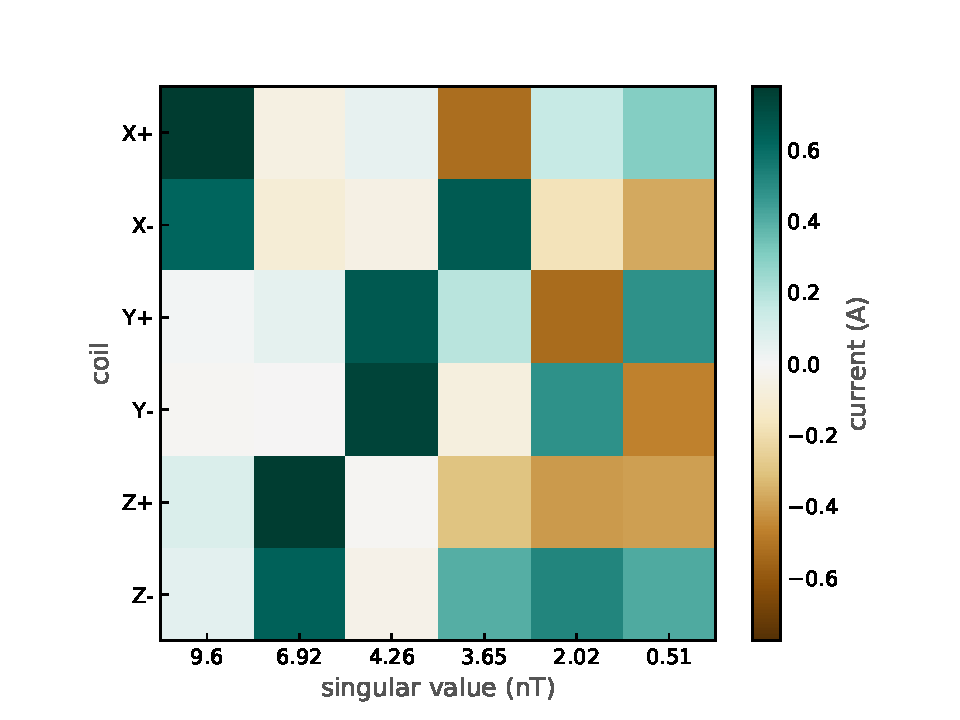
\includegraphics[width=.8\linewidth]{gfx/nEDM_SFC/coil-singular_vectors_of_the_nEDM_SFC_matrix.pdf}
  \caption{The coil-singular values of the SFC matrix. Columns correspond to singular combinations of the coils (labeled as in Fig.\,\ref{fig:sfc-scheme}). For each column the corresponding singular value is indicated.}\label{fig:nEDM_SFC_svd}
\end{figure}

Figure~\ref{fig:nEDM_SFC_svd} presents the spectrum of the PSI's SFC feedback matrix. The condition number is $9.6 / 0.51 = 18.2$. A factor of 18 amplification of noise points to why the regularisation was necessary.

It is interesting to ask \emph{why} the system had an ill-defined feedback matrix. A very small singular value means that there exists a coil, or a combination thereof, which has about 18 times smaller influence on the field then other ones. In Fig.\,\ref{fig:nEDM_SFC_svd} the columns are the singular values with their corresponding coil-vectors. The first three, starting from the left, are easiest to interpret. Each of them is a pair of coils configured as Helmholtz-pair with roughly the same current, producing a homogeneous field in each of the spatial directions.
%The smaller singular value, or the effect on the field, in the Y direction is explained by the fact that this is the longitudinal axis of the μ-metal cylinder.
The last column has also a clear interpretation: it corresponds to all pairs configured as anti-Helmholtz---currents flowing in the opposite directions in each pair. The magnetic field that was created by such a configuration was complicated and high-order. The fact that this combination has so little influence on the measured field means that it hardly changes any solution for currents when added to it. It spans a valley in the parameter space in the least-squares problem. If not regularised, a small change in the measured field would cause a large change in the currents along the valley. Rapid oscillations in this direction would render the system unstable.

An important observation is that the feedback matrix is defined solely by the configuration of the coils, sensors and ferromagnetic materials. It follows that already at the design stage one can, and should, take care about the definiteness of the system.

% \note{Propose here immediately a solution: orthogonal system for elements of expansion! Any combination of 1st order gradients is a 1st order gradient.}




\section{Design challenges for n2EDM}
\label{sec:n2EDM_challenges}
There was relatively a lot of space available around the passive magnetic shield of the nEDM experiment at PSI (see Fig.\,\ref{fig:sfc-scheme}).
The SFC system exploited that space by making the coils much larger than the shield.
However, the successor experiment, n2EDM, was going to have a much larger passive magnetic shield.
Spatial constraints were a major concern in the design of coils of a new active shield.

 Assume, that all there is to compensate are homogeneous fields.
 That is the zeroth order approximation concerning the space expansion of the magnetic field.
 To compensate them, a system needs to have coils that can produce a homogeneous field.
 Yet, the volume where the field of a coil system is homogeneous is limited.
 For example, in a case of a Helmholtz pair, the (linear) size of the volume where the generated field is homogeneous on a \SI{2}{\percent} level is only around \num{0.4} that of the (linear) size of the coils.
 Increasing the relative size of the homogeneous volume requires more elaborate designs~\cite{Kirschvink1992}.
 When three Helmholtz pairs are used to compensate a homogeneous change, they only do so inside this limited volume.
 Outside, the field may even be more unstable, the extreme case being right next to the coils, where the field can get arbitrarily large.
 The situation is similar for any type of field: an active shield can only stabilise the field in a limited volume.

\begin{figure}
  \centering
  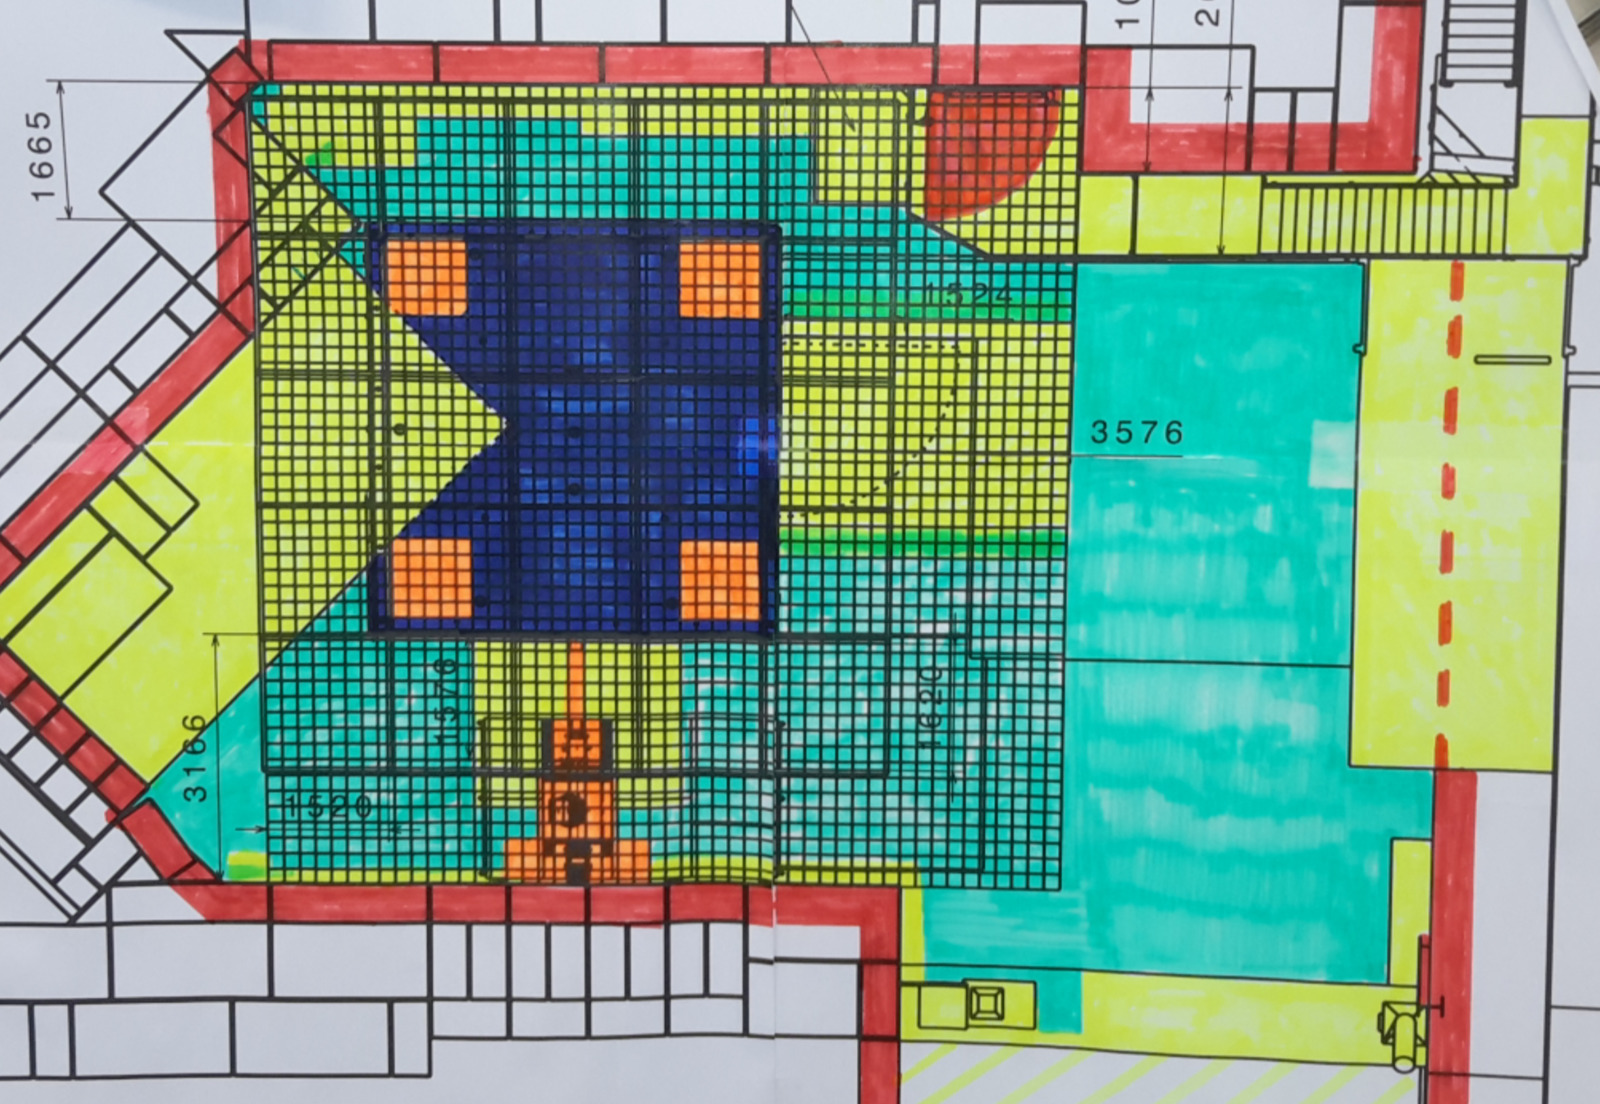
\includegraphics[width=\linewidth]{gfx/nEDM_SFC/n2EDM_SFC_situation.png}
  \caption{A plan by Michael Meier highlighting the potential conflicts between coils of an n2EDM active shield and other structures. The vicinity of the biological shielding (red) forced the coils to be designed relatively close to the magnetic shield (dark blue). Other bodies, like the support legs of the passive shield (orange), polarising magnet (orange) and an emergency exit from a nearby accelerator (red) gave additional constraints.}\label{fig:n2EDM_sfc_situational_plan}
\end{figure}

Figure~\ref{fig:n2EDM_sfc_situational_plan} depicts the major spatial constraints in the design of the n2EDM active shield.
Firstly, the passive shield was going to be \SI{5}{\metre} large in each direction, with the available space being $\approx \SI{7.5}{\metre}$ (a ratio of \num{0.7}).
In nEDM the shield was around \SI{2}{\meter} and the SFC coils \SIrange[range-phrase = --, range-units=single]{6}{8}{\meter} (a ratio of around \num{0.3}).
Secondly, other bodies put additional constraints (Fig.\,\ref{fig:n2EDM_sfc_situational_plan}): support legs of the passive shield, the polarising magnet and an emergency exit from a nearby cyclotron.

For the design of the n2EDM active shield it was necessary to come up with coils that could produce such a field, that they are likely to compensate, and do that in the whole volume occupied by the shield. Unfortunately, because of spatial constraints no known design could be used~\cite{Turner1986,Wong1991,Turner1993,Crozier1993,Sanchez2007,Sanchez2009}. This, together with a concern about ensuring a low condition number of the system, called for an in-depth investigation into the geometry of the future system's coils, which led to the development of a new approach to magnetic field coils design---the topic of the next chapter.

% Some came from the experimental hall itself. For example an emergency exit from a nearby accelerator and a staircase leading to it (see Fig.\,\ref{fig:n2EDM_sfc_situational_plan}). Other constraints were due to higher-priority components of the experiment itself: legs on which the shield stands, the magnet used to polarise the neutrons, the neutron detection system, and the door of the magnetic shield.
